%! TeX program = lualatex
%---------------------------ALLGEMEINE IMPORTS-------------------------------------
\documentclass[12pt,english,ngerman]{scrartcl}
\input{./protokoll_template/template.latex/input/shared_preamble.tex}

% Kopfzeile
\ihead{WS22\\
	09.12.2022} \chead{\textsc{Stark} Matthias - 12004907 \\
	\textsc{Philipp} Maximilian - 11839611}
\ohead{FLAB 1 \\
	Leistungsmessung}
% Fußzeile
\addbibresource{leistungsmessung.bib}

\begin{document}
%todo deckblatt
%\includepdf{./deckblatt3.pdf}
\tableofcontents
\newpage

\section{Aufgabenstellung\label{Auf}}

\begin{itemize}
	\item Leistungsmessung einer ohmschen Last in einem Wechselstromkreis
	\item Wirkleistungsmessung im Drehstromnetz bei einer symmetrischen ohmschen Last in
	      Stern- und Dreieckschaltung mit Aronschaltung
	\item Wirk- und Blindleistungsmessung bei einer allgemeinen Last im Dreiphasennetz
	\item Bauen eines rudimentärern Asynchron-Drehstrommotors
\end{itemize}

\section{Grundlagen}\label{Grund}

Für die Wirkleistung $P$ eines ohmschen Verbrauchers gilt unter Verwendung des
Ohmschen Gesetzes, \autoref{eq:ohmschesgesetz}, folgender Zusammenhang:

\begin{equation}
	P = U \cdot I = I^2 \cdot R = \frac{U^2}{R}
	\label{eq:wirkleistung}
\end{equation}

\begin{equation}
	U = R \cdot I
	\label{eq:ohmschesgesetz}
\end{equation}

Dabei Beschreibt $U$ die Spannung, $I$ die Stromstärke und $R$ den ohmschen
Widerstand.

Werden im Wechselstromkreis nun Spulen oder Kondensatoren betrachtet, empfiehlt
es sich komplexe Zahlen einzuführen, da hier die Impedanz $Z$ betrachtet werden
muss, die sich nach folgender Formel berechnet:

\begin{equation}
	Z = R + iX
	\label{eq:Impedanz}
\end{equation}

$R$ bezeichnet dabei den Realteil des Widerstands der entsprechenden Last und $X$ die entsprechende Reaktanz.
Diese kann für Induktivitäten, $X_L$, und Kapazitäten, $X_C$, folgendermaßen berechnet werden:

\begin{equation}
	X_L = i\omega L
	\label{eq:Reaktanzl}
\end{equation}

\begin{equation}
	X_C = - \frac{i}{\omega C}
	\label{eq:Reaktanzc}
\end{equation}

$L$ steht dabei für die Induktivität der Spule, $C$ für die Kapazität des Kondensators und $\omega$ für die
vorliegende Frequenz des Wechselstroms.

Mit der eingeführten Größe der Impedanz $Z$ kann nun das ohmsche Gesetz
folgendermaßen verallgemeinert werden:

\begin{equation}
	U = Z \cdot I
	\label{eq:ohmschesgesetz_z}
\end{equation}

Die komplexen Spannungen und Ströme werden am übersichtlichsten in einem
Zeigerdiagramm dargestellt. Dazu empfiehlt sich folgende Schreibweise:

\begin{equation}
	\underline{U} = U_{\textrm{eff}} \cdot e^{i(\omega t + \phi U)}
	\label{eq:komplexespannung}
\end{equation}

\begin{equation}
	\underline{I} = I_{\textrm{eff}} \cdot e^{i(\omega t + \phi I)}
	\label{eq:komplexerstrom}
\end{equation}
$U_{\textrm{eff}}$ und $I_{\textrm{eff}}$ entsprechen dabei der jeweiligen Größe, wenn sie ein rein ohmsche Verbraucher, ohne
komplexe Anteile, wäre.

Dadurch kann die erhaltene Wirkleistung $P$ folgendermaßen ausgedrückt werden:

\begin{equation}
	P = \textrm{Re}(\underline{U}\underline{I}^*)
	\label{eq:wirkleistung}
\end{equation}

Weiters können auch die vom System tatsächlich aufgewendete Scheinleistung,
$S$, und die nicht nutzbare Blindleistung, $Q$, berechnet werden.

\begin{equation}
	S = \sqrt[]{\underline{U}\underline{U}^*\underline{I}\underline{I}^*}
	\label{eq:scheinleistung}
\end{equation}

\begin{equation}
	Q = \textrm{Re}(\underline{U}\underline{I}^*)
	\label{eq:blindleistung}
\end{equation}

%todo max schau amol ob die Grundlagen dir so passen weil es steht extra drin 1-1.5 Seiten also wollt i nit mehr schreiben

\section{Versuchsanordnung}
\label{sec:versuchsanordnung}

\subsection{ohmsche Last in Wechselstromkreis}

Um die ohmsche Last einer Glühlampe im Wechselstromkreis zu messen, wird
folgender Versuchsaufbau aus \autoref{fig:aufbau_ohm} realisiert.

\begin{figure}[H]
	\begin{center}
		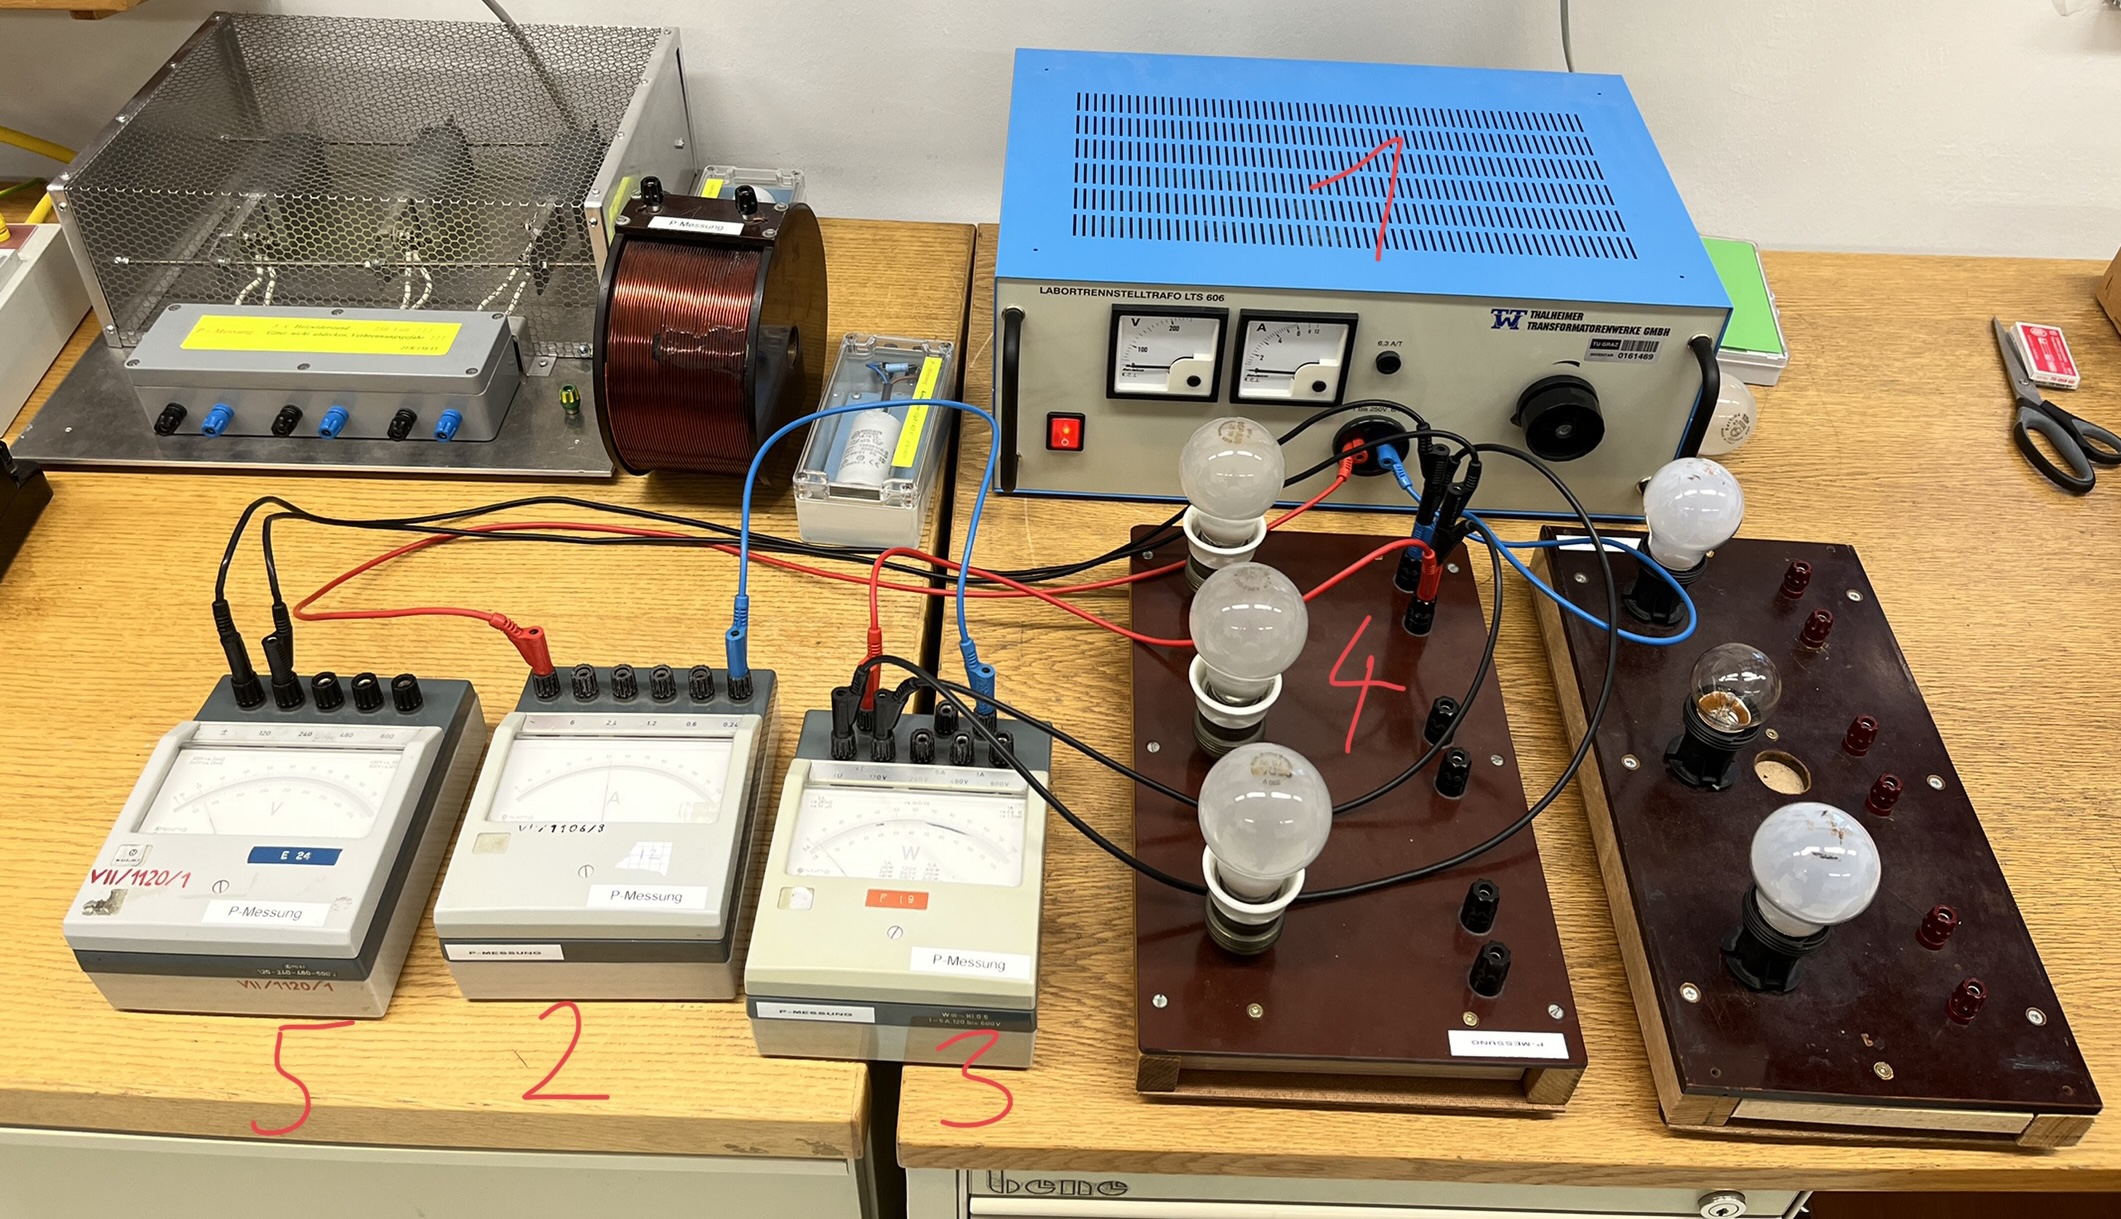
\includegraphics[width = 0.5\textwidth]{./figures/aufbau_ohm.png}
	\end{center}
	\caption[Realer Versuchsaufbau für die Messung einer ohmschen Last] {Realer
		Versuchsaufbau für die Messung einer ohmschen Last \\
		1 \(\dots\) Transformator                          \\
		2 \(\dots\) seriell geschaltetes Strommessgerät    \\
		3 \(\dots\) seriell geschaltetes Leistungsmessgerät mit parallelen Anschluss
		zum Verbraucher                                    \\
		4 \(\dots\) ohmscher Verbraucher (Glühlampe)       \\
		5 \(\dots\) parallel geschaltetes Spannungsmessgerät
	}\label{fig:aufbau_ohm}
\end{figure}

\subsection{Symmetrische Last in Dreieckschaltung}

Um die Wirkleistung von symmetrischen Verbrauchern in einer Dreiecksschaltung
zu Messen, wird die Aronschaltung nach folgendem Schaltplan aus
\autoref{fig:aufbau1} realisiert. Der tatsächliche Versuchsaufbau ist in
\autoref{fig:aufbau1_echt} ersichtlich.

\begin{figure}[H]
	\begin{center}
		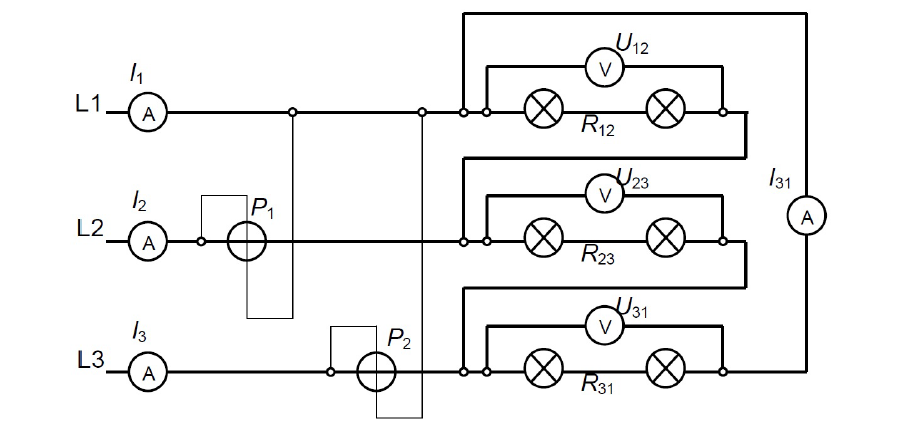
\includegraphics[width = 0.8\textwidth]{./figures/aufbau1.png}
	\end{center}
	\caption[Schaltplan für die Messung der Wirkleistung mit Aronschaltung für symmetrische
		Verbraucher in Dreiecksschaltung] {Schaltplan für die Messung der Wirkleistung
		mit Aronschaltung für symmetrische Verbraucher in
		Dreiecksschaltung~\cite[]{leistungsmessungvorbereitung}                          \\
		$I_i$ \(\dots\) entsprechende Ströme gemessen mit entsprechenden Amperemeter A   \\
		$U_i$ \(\dots\) entsprechende Spannungen gemessen mit entsprechenden Voltmeter V \\
		$R_i$ \(\dots\) entsprechender Widerstand durch die jeweiligen Verbraucher       \\
		$P_i$ \(\dots\) Powermeter in Aronschaltung
	}\label{fig:aufbau1}
\end{figure}

\begin{figure}[H]
	\begin{center}
		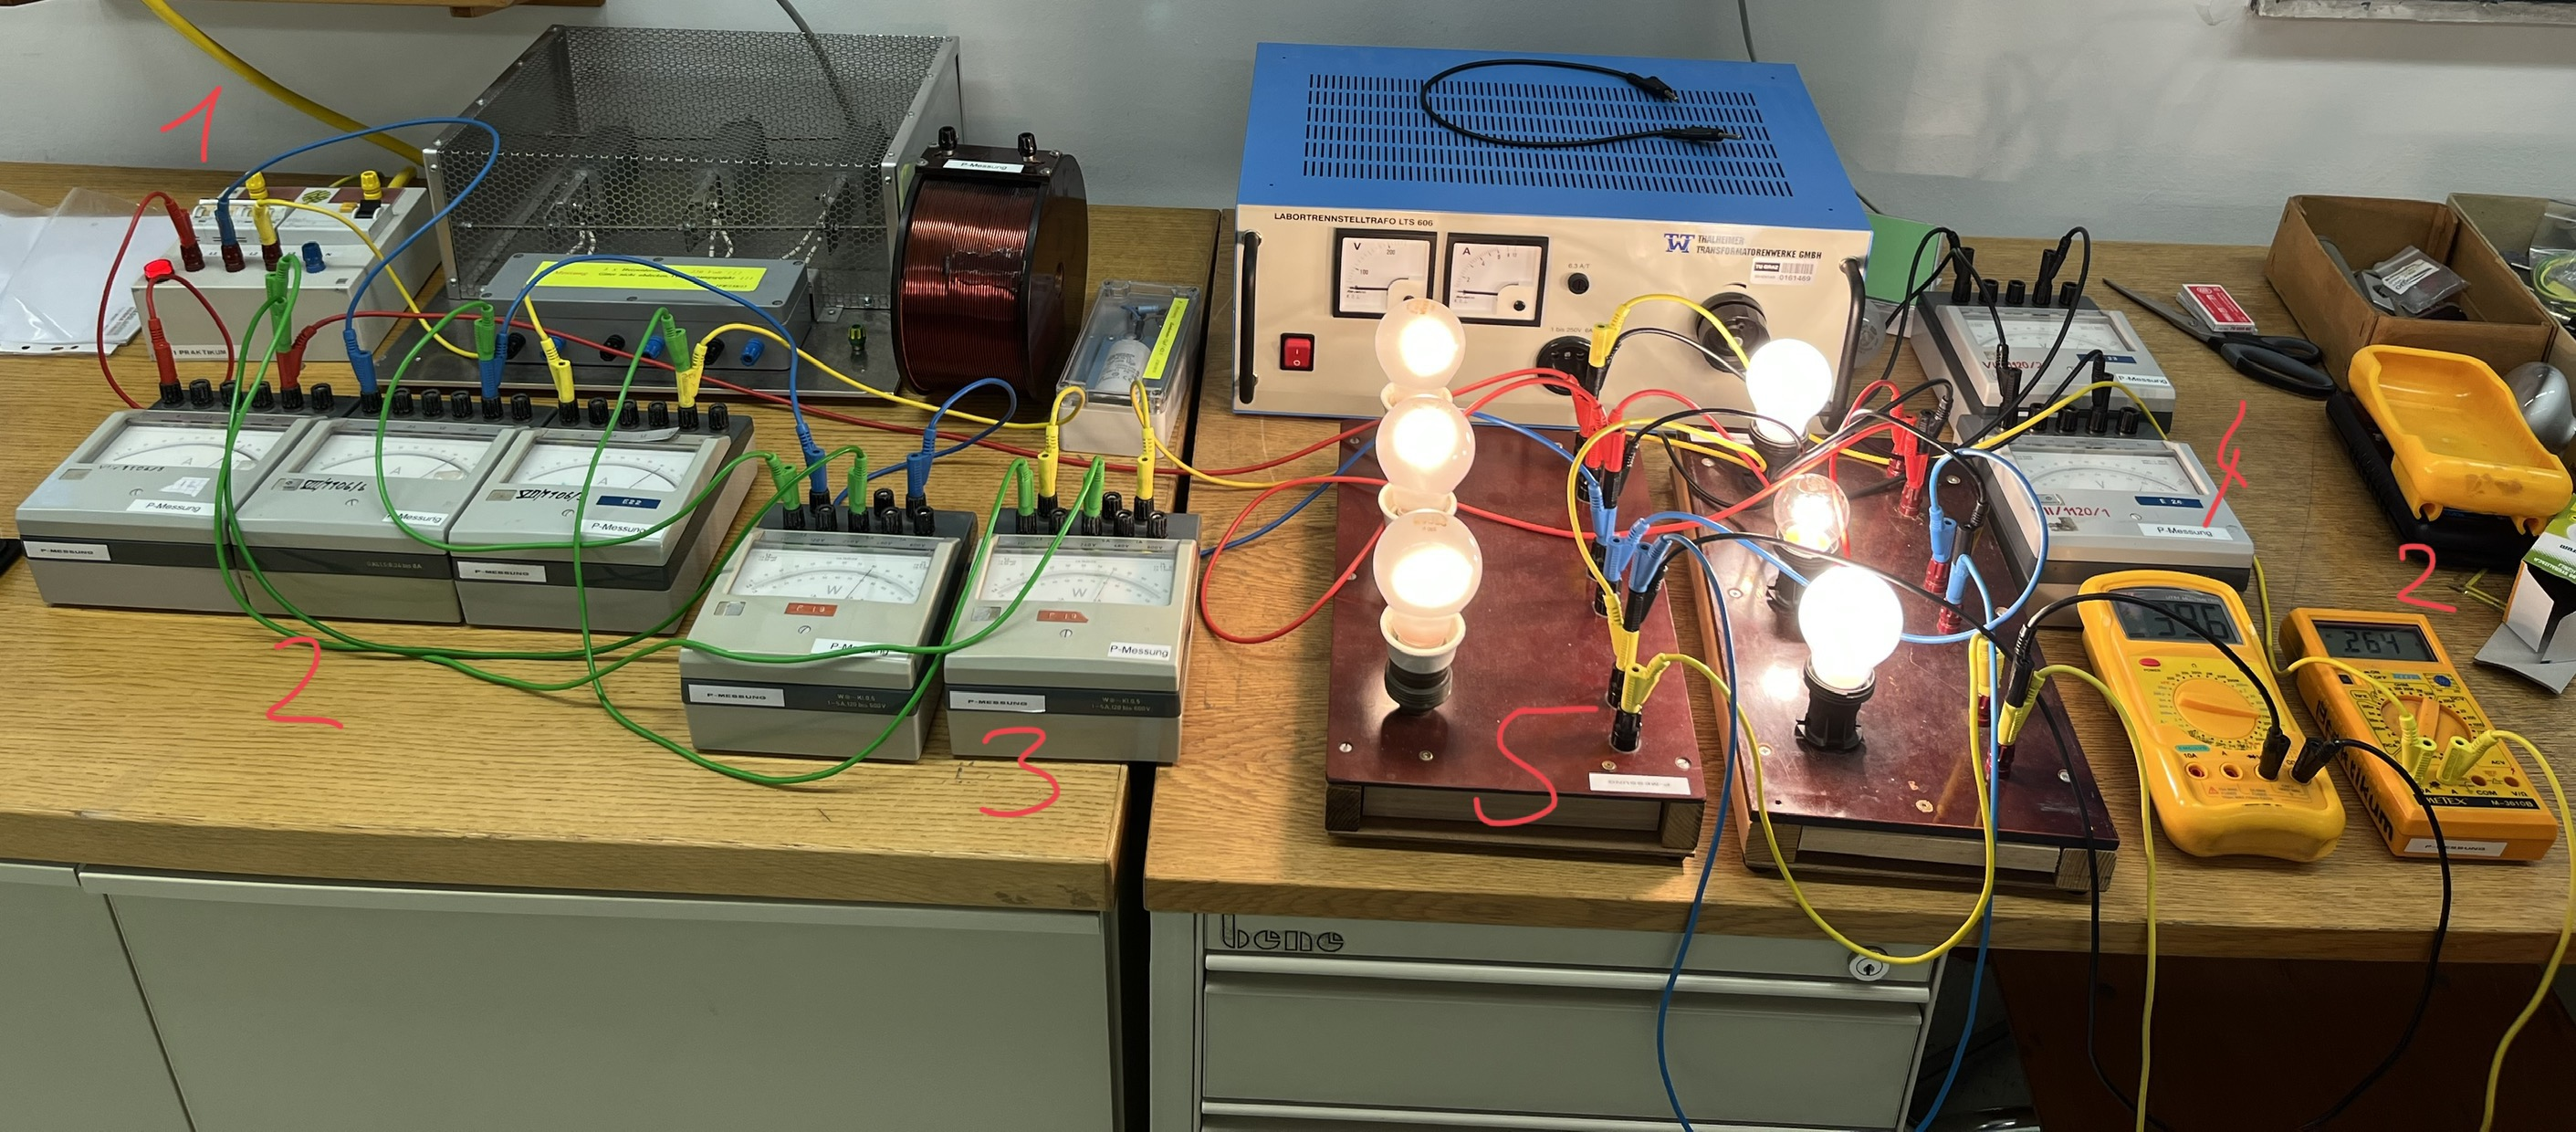
\includegraphics[width = \textwidth]{./figures/aufbau1_echt.png}
	\end{center}
	\caption[Realer Versuchsaufbau für die Messung der Wirkleistung mit Aronschaltung für
		symmetrische Verbraucher in Dreiecksschaltung] {Realer Versuchsaufbau für die
		Messung der Wirkleistung mit Aronschaltung für symmetrische Verbraucher in
		Dreiecksschaltung. (Bei den Kabeln wurde ein Farbschema eingehalten, um eine
		bessere Übersicht zu ermöglichen.)                                  \\
		1 \(\dots\) Versorgungsspannung ($L_1$ rot, $L_2$ blau, $L_3$ gelb) \\
		2 \(\dots\) seriell geschaltete Strommessgeräte                     \\
		3 \(\dots\) seriell geschaltete Leistungsmessgeräte mit parallelen Anschlüssen
		nach der Aronschaltung (grün)                                       \\
		4 \(\dots\) parallel geschaltete Spannungsmessgeräte über die entsprechenden
		Verbraucher (schwarz)                                               \\
		5 \(\dots\) symmetrisch verteilte ohmsche Verbraucher (Glühlampen)
	}
	\label{fig:aufbau1_echt}
\end{figure}

\subsection{Symmetrische Last in Sternschaltung}

Um die Wirkleistung von symmetrischen Verbrauchern in einer Sternschaltung zu
Messen, wird die Aronschaltung nach folgendem Schaltplan aus
\autoref{fig:aufbau2} realisiert. Der tatsächliche Versuchsaufbau ist in
\autoref{fig:aufbau2_echt} ersichtlich.

\begin{figure}[H]
	\begin{center}
		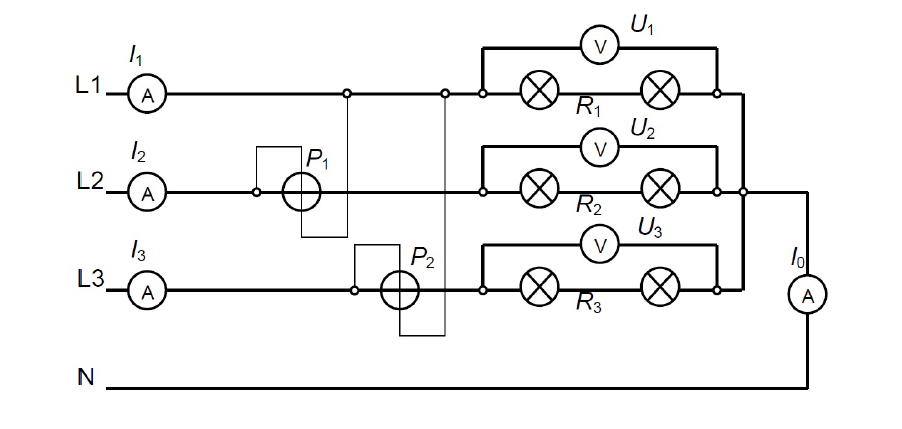
\includegraphics[width = 0.8\textwidth]{./figures/aufbau2.png}
	\end{center}
	\caption[Schaltplan für die Messung der Wirkleistung mit Aronschaltung für symmetrische
		Verbraucher in Sternschaltung] {Schaltplan für die Messung der Wirkleistung mit
		Aronschaltung für symmetrische Verbraucher in
		Sternschaltung~\cite[]{leistungsmessungvorbereitung}                             \\
		$I_i$ \(\dots\) entsprechende Ströme gemessen mit entsprechenden Amperemeter A   \\
		$U_i$ \(\dots\) entsprechende Spannungen gemessen mit entsprechenden Voltmeter V \\
		$R_i$ \(\dots\) entsprechender Widerstand durch die jeweiligen Verbraucher       \\
		$P_i$ \(\dots\) Powermeter in Aronschaltung
	}
	\label{fig:aufbau2}
\end{figure}

\begin{figure}[H]
	\begin{center}
		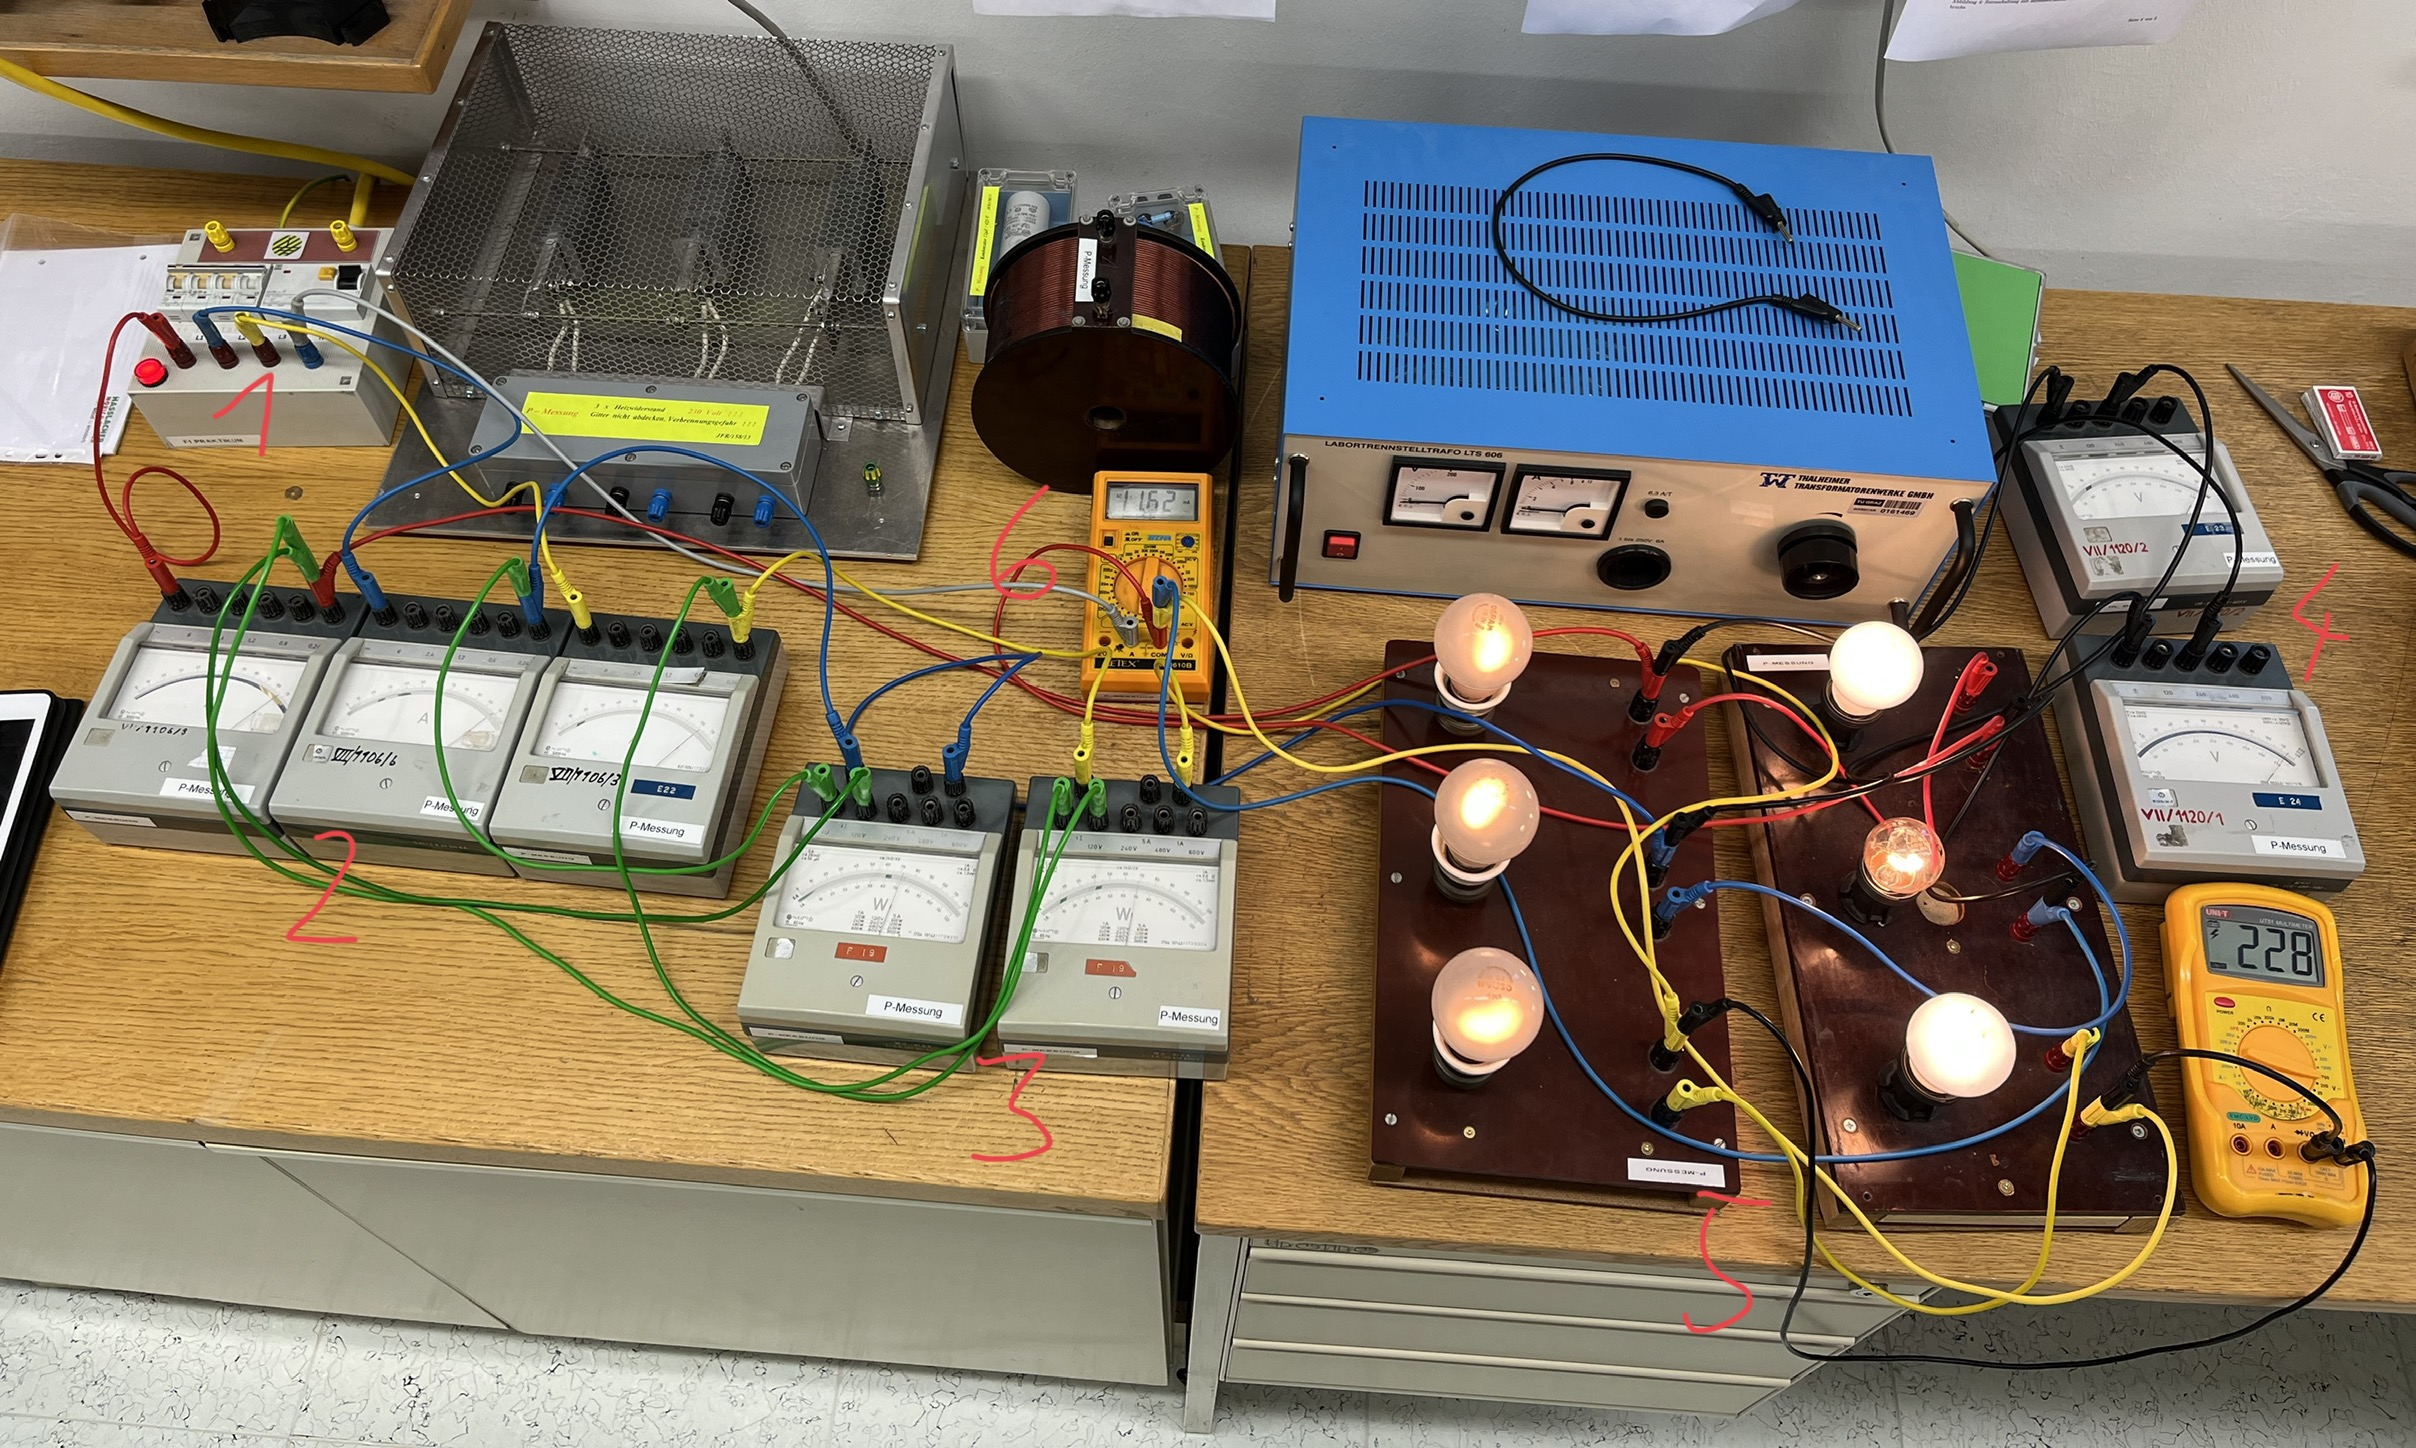
\includegraphics[width = \textwidth]{./figures/aufbau2_echt.png}
	\end{center}
	\caption[Realer Versuchsaufbau für die Messung der Wirkleistung mit Aronschaltung für
		symmetrische Verbraucher in Sternschaltung] {Realer Versuchsaufbau für die
		Messung der Wirkleistung mit Aronschaltung für symmetrische Verbraucher in
		Sternschaltung. (Bei den Kabeln wurde ein Farbschema eingehalten, um eine
		bessere Übersicht zu ermöglichen.)                                  \\
		1 \(\dots\) Versorgungsspannung ($L_1$ rot, $L_2$ blau, $L_3$ gelb) \\
		2 \(\dots\) seriell geschaltete Strommessgeräte                     \\
		3 \(\dots\) seriell geschaltete Leistungsmessgeräte mit parallelen Anschlüssen
		nach der Aronschaltung (grün)                                       \\
		4 \(\dots\) parallel geschaltete Spannungsmessgeräte über die entsprechenden
		Verbraucher (schwarz)                                               \\
		5 \(\dots\) symmetrisch verteilte ohmsche Verbraucher (Glühlampen)  \\
		6 \(\dots\) Strommessgerät zwischen Sternpunkt und Neutralleiter (grau)
	}\label{fig:aufbau2_echt}
\end{figure}

\subsection{Asymmetrische Last in Sternschaltung}

Um eine asymmetrische Last zu erreichen, wird der Aufbau aus
\autoref{fig:aufbau2} herangezogen, mit dem Unterschied, dass die Glühlampen
nicht gleichmäßig auf die Leiter aufgeteilt werden. Die gewählte Konfiguration
ist in \autoref{fig:lampenasym} ersichtlich.

\begin{figure}[H]
	\begin{center}
		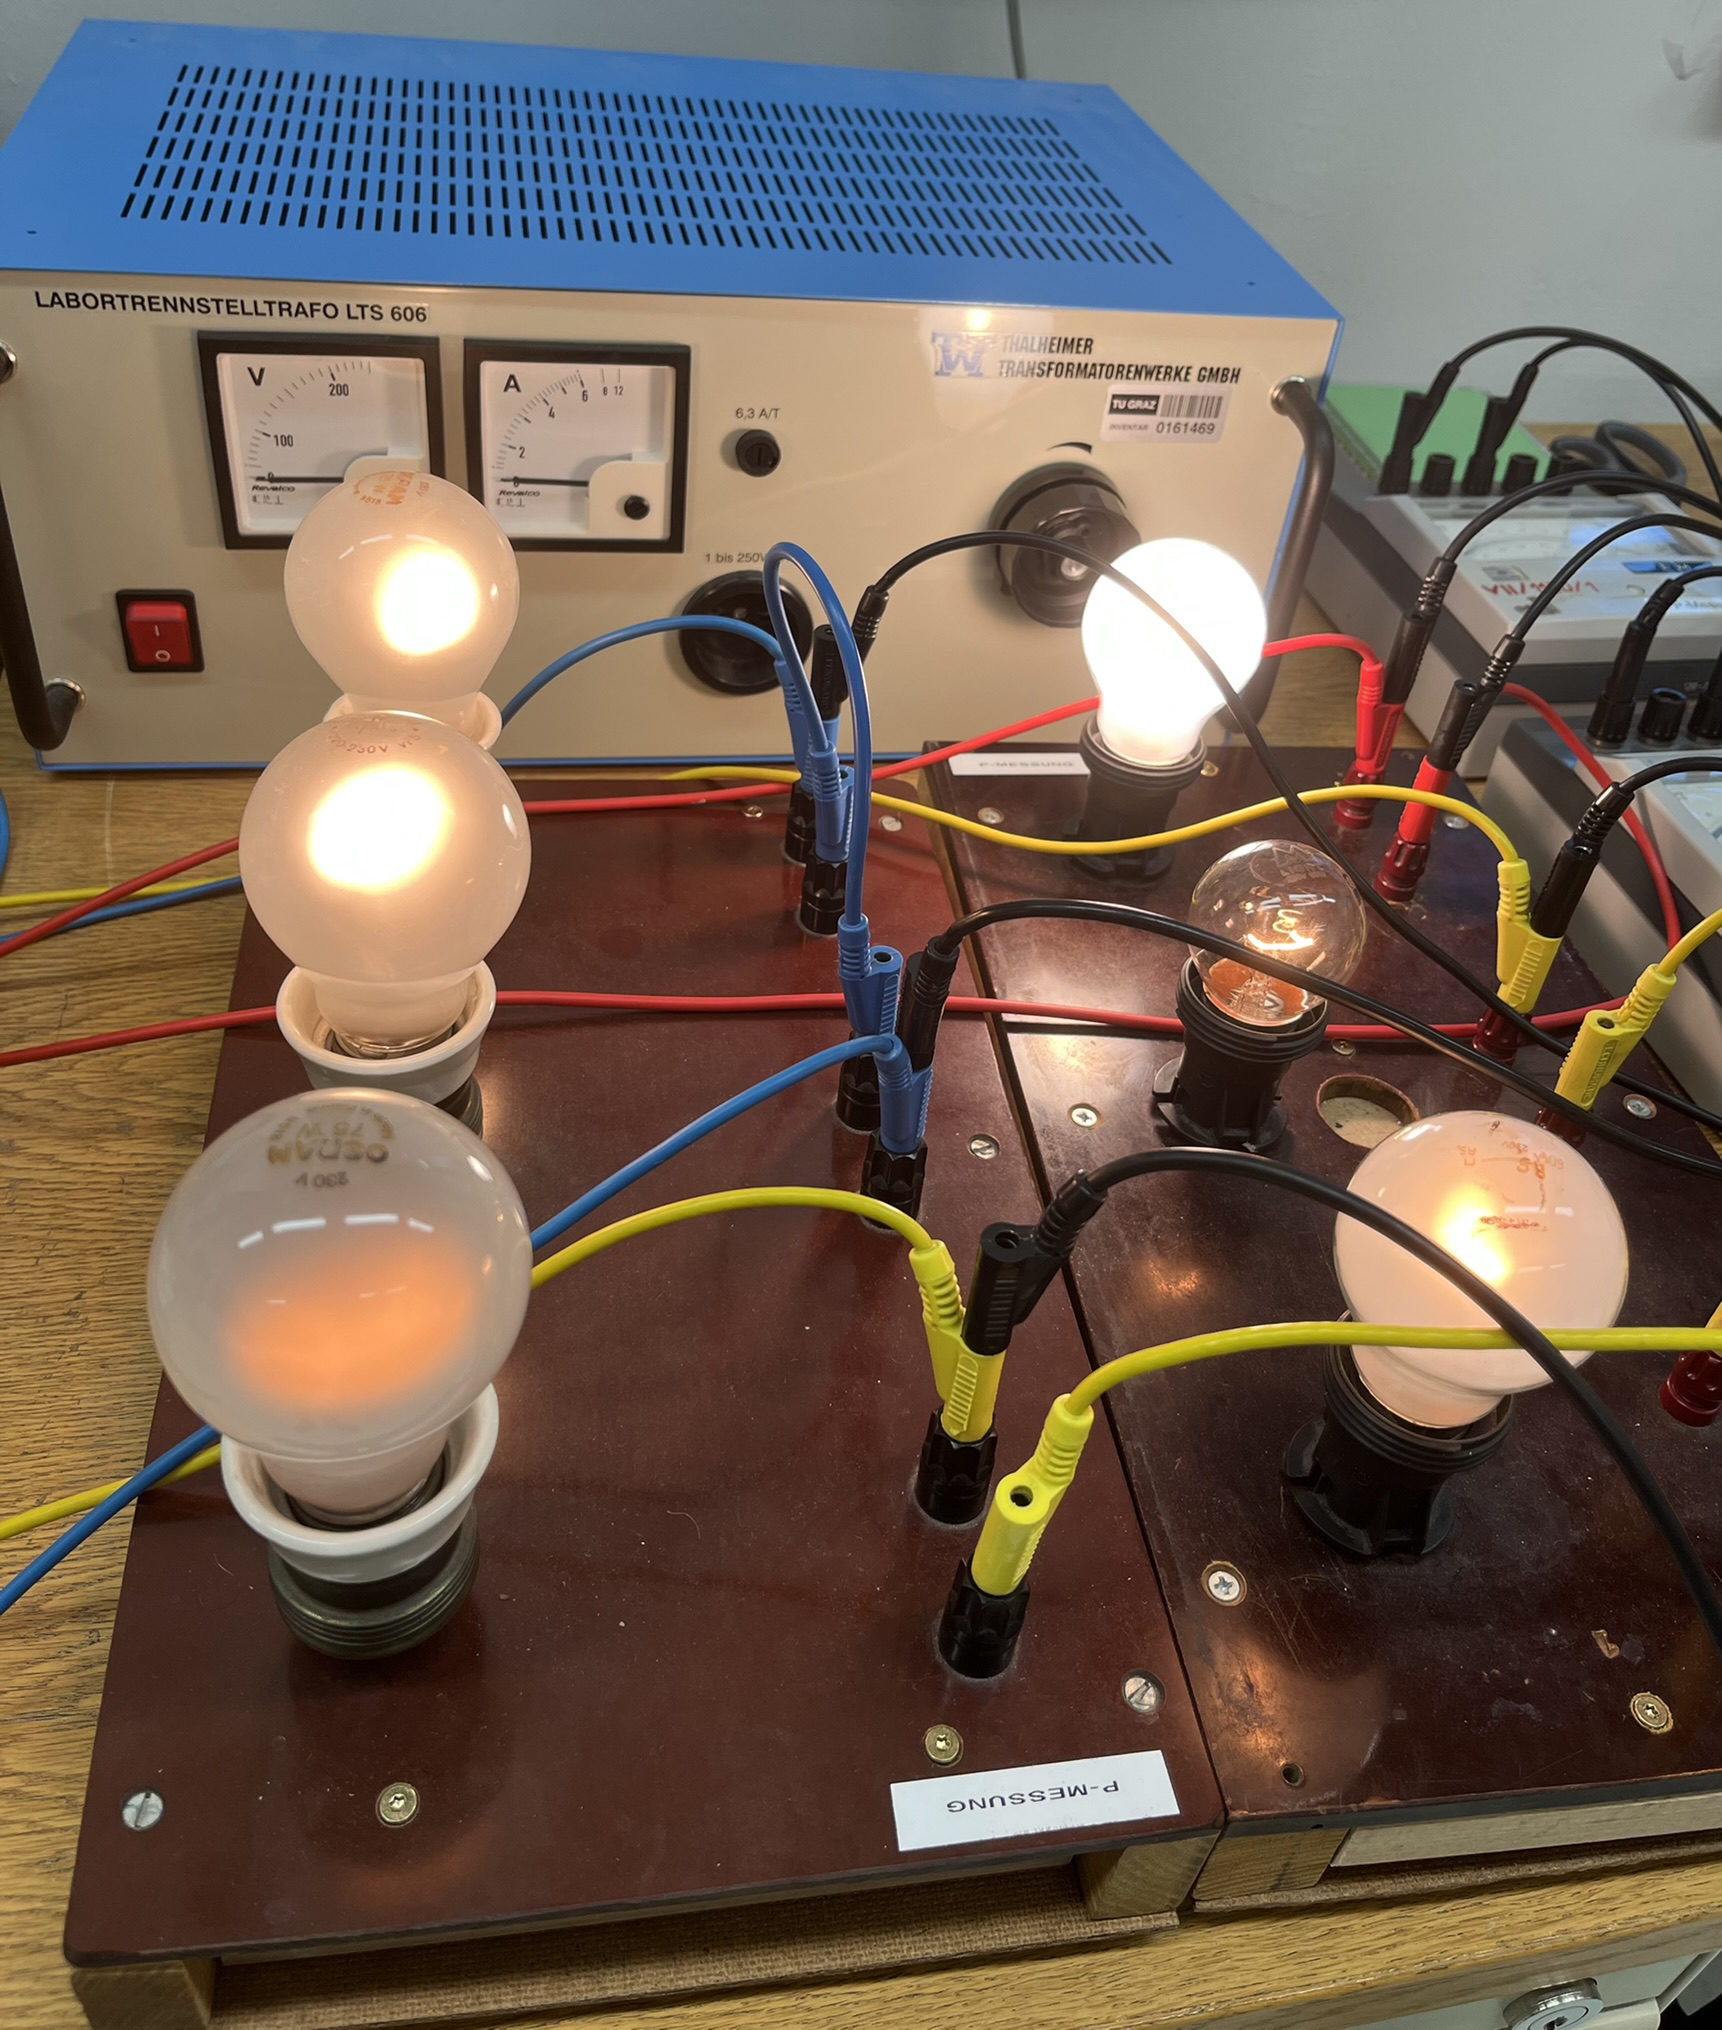
\includegraphics[width = 0.5\textwidth]{./figures/lampen.png}
	\end{center}
	\caption[Entsprechende Konfiguration für eine asymmetrische Verteilung der Last]
	{Entsprechende Konfiguration für eine asymmetrische Verteilung der Last mit
		folgenden Verteilungen auf den Strängen: \\
		$L_1$ \(\dots\) 1 x \SI[]{60}{\watt}     \\
		$L_2$ \(\dots\) 2 x \SI[]{75}{\watt}     \\
		$L_3$ \(\dots\) 1 x \SI[]{75}{\watt} und 2 x \SI[]{60}{\watt}
	}\label{fig:lampenasym}
\end{figure}

\subsection{Asymmetrische Last in Sternschaltung und simulierten Kabelbruch}

Um einen Kabelbruch zu simulieren, wird der Aufbau aus \autoref{fig:aufbau2}
herangezogen. Nun wird der Kontakt des Neutralleiters unterbrochen, indem das
graue Kabel, sichtbar in \autoref{fig:aufbau1_echt}, aus dem Strompfad des
Multimeters entfernt und in den Spannungsbereich gesteckt wird, um eine
Spannungsmessung zu ermöglichen.

\subsection{Wirkleistungsmessung}

Um die Wirkleistung von allgemeinen Verbrauchern in Sternschaltung zu
bestimmen, wird die Schaltung nach folgendem Schaltplan aus
\autoref{fig:aufbau3} aufgebaut. Der tatsächliche Versuchsaufbau ist in
\autoref{fig:aufbau3_echt} ersichtlich.

\begin{figure}[H]
	\begin{center}
		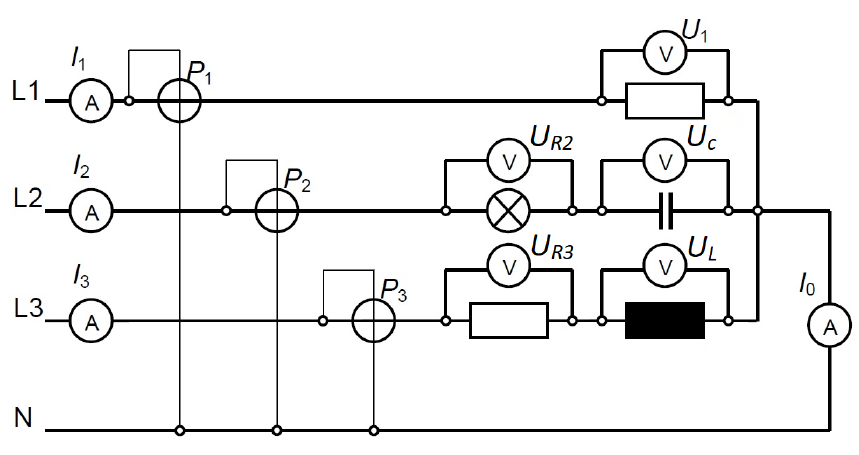
\includegraphics[width = 0.8\textwidth]{./figures/aufbau3.png}
	\end{center}
	\caption[Schaltplan für die Messung der Wirkleistung für allgemeine Verbraucher in
		Sternschaltung] {Schaltplan für die Messung der Wirkleistung für allgemeine
		Verbraucher in Sternschaltung~\cite[]{leistungsmessungvorbereitung}              \\
		$I_i$ \(\dots\) entsprechende Ströme gemessen mit entsprechenden Amperemeter A   \\
		$U_i$ \(\dots\) entsprechende Spannungen gemessen mit entsprechenden Voltmeter V \\
		$R_i$ \(\dots\) entsprechender Widerstand durch die jeweiligen Verbraucher       \\
		$P_i$ \(\dots\) Powermeter
	}
	\label{fig:aufbau3}
\end{figure}

\begin{figure}[H]
	\begin{center}
		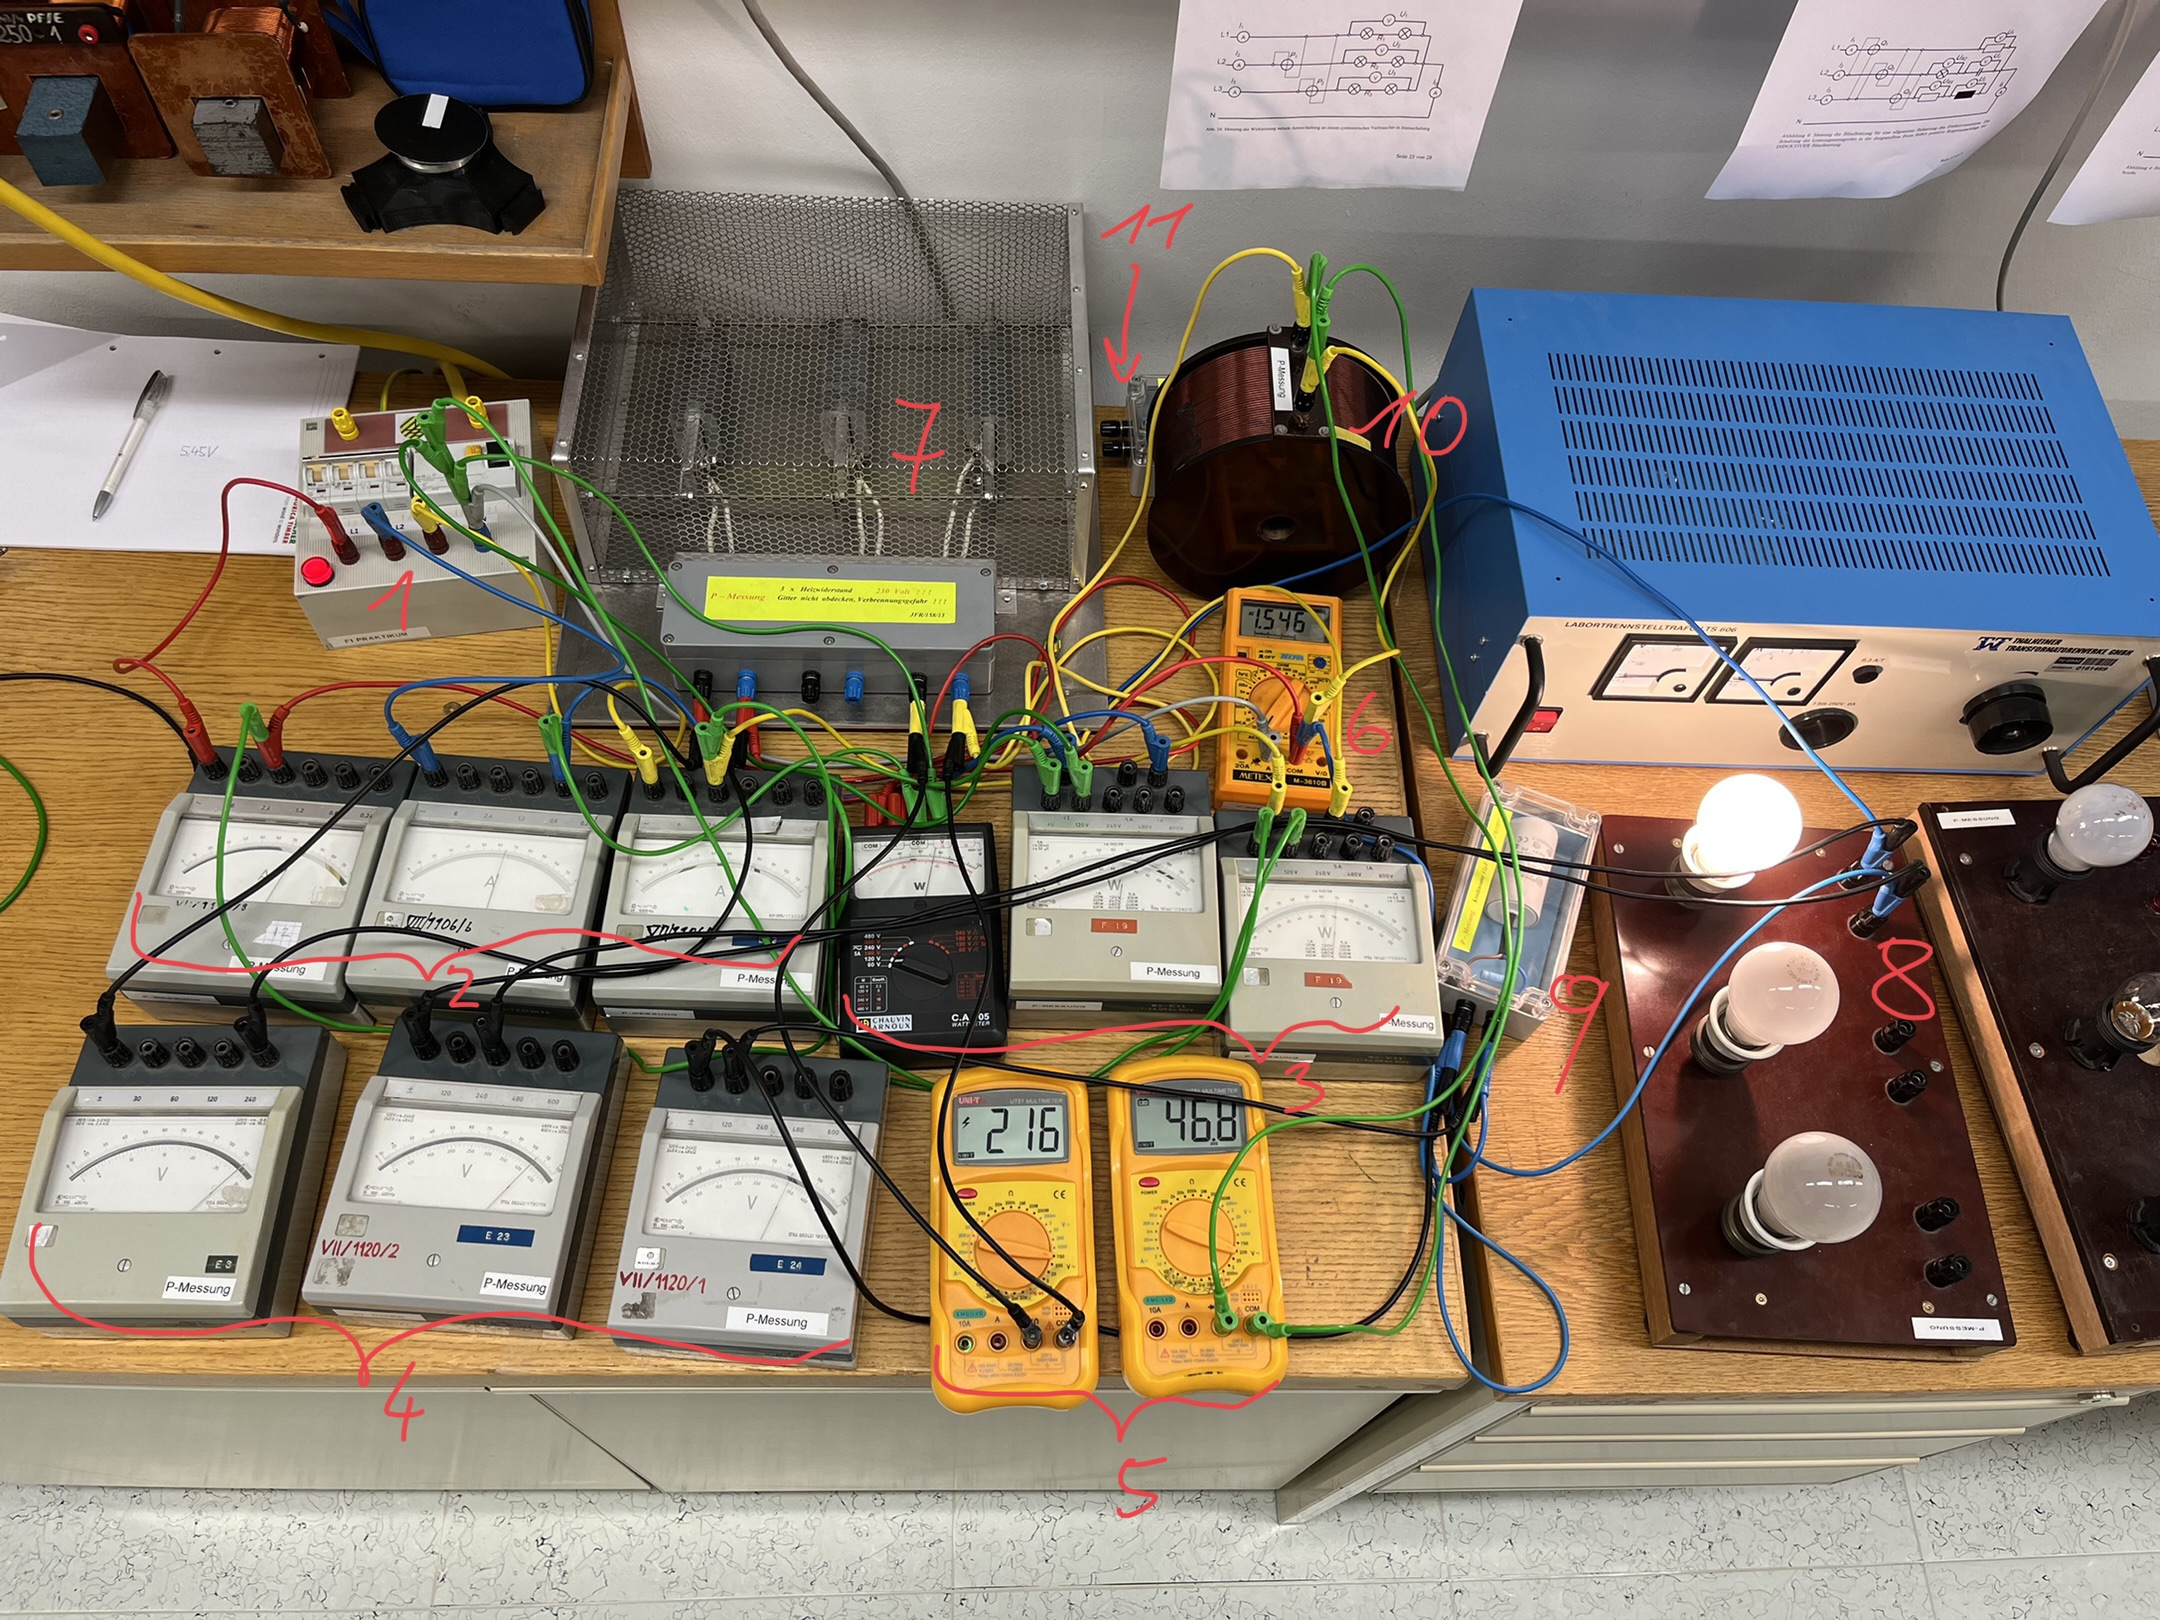
\includegraphics[width = \textwidth]{./figures/aufbau3_echt.png}
	\end{center}
	\caption[Realer Versuchsaufbau für die Messung der Wirkleistung für allgemeine
		Verbraucher in Sternschaltung] {Realer Versuchsaufbau für die Messung der
		Wirkleistung für allgemeine Verbraucher in Sternschaltung. (Bei den Kabeln
		wurde ein Farbschema eingehalten, um eine bessere Übersicht zu ermöglichen.) \\
		1 \(\dots\) Versorgungsspannung ($L_1$ rot, $L_2$ blau, $L_3$ gelb)          \\
		2 \(\dots\) seriell geschaltete Strommessgeräte                              \\
		3 \(\dots\) seriell geschaltete Leistungsmessgeräte mit parallelen Anschlüssen
		zum Neutralleiter (grün)                                                     \\
		4 \(\dots\) parallel geschaltete analoge Spannungsmessgeräte über die
		entsprechenden Verbraucher (schwarz)                                         \\
		5 \(\dots\) parallel geschaltete digitale Spannungsmessgeräte über die
		entsprechenden Verbraucher (schwarz/grün)                                    \\
		6 \(\dots\) Strommessgerät zwischen Sternpunkt und Neutralleiter (grau)      \\
		7 \(\dots\) Heizwiderstände                                                  \\
		8 \(\dots\) ohmscher Verbraucher                                             \\
		9 \(\dots\) Kapazität (Kondensator)                                          \\
		10 \(\dots\) Induktivität (Spule)                                            \\
		11 \(\dots\) 2. Kapazität für Bonusaufgabe

	}\label{fig:aufbau3_echt}
\end{figure}

Für die Bonusaufgabe werden folgende Änderungen vorgenommen:

\begin{itemize}
	\item $L_1$ bleibt unverändert (Heizwiderstand)
	\item $L_2$ Schaltung von einem Heizwiderstand und einem Kondensator mit parallel geschalteter Induktivität
	\item $L_3$ Schaltung von einem Heizwiderstand und einem Kondensator
\end{itemize}

\subsection{Blindleistungsmessung}

Um die Blindleistung eines allgemeinen Verbrauchers sichtbar zu machen, wird
nun die Schaltung nach folgendem Schaltplan aus \autoref{fig:aufbau4}
aufgebaut, indem die grünen Kabel der Powermeter aus \autoref{fig:aufbau3_echt}
entsprechend modifiziert werden.

\begin{figure}[H]
	\begin{center}
		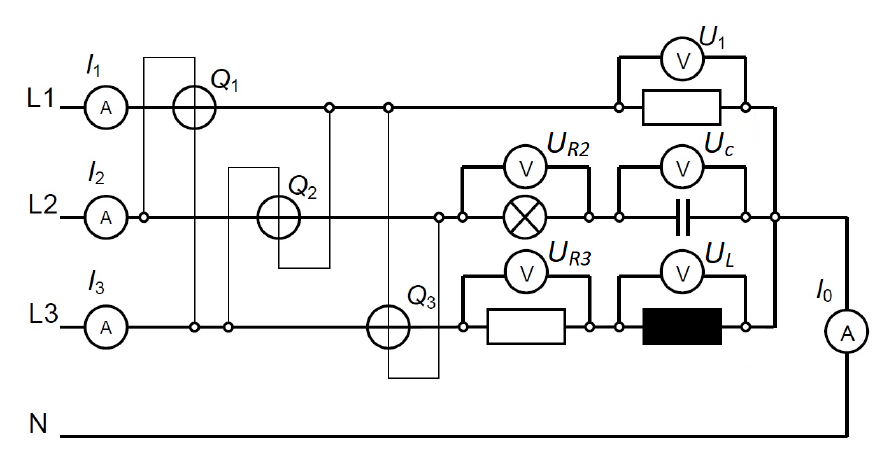
\includegraphics[width = 0.8\textwidth]{./figures/aufbau4.png}
	\end{center}
	\caption[Schaltplan für die Messung der Blindleistung für allgemeine Verbraucher in
		Sternschaltung] {Schaltplan für die Messung der Blindleistung für allgemeine
		Verbraucher in Sternschaltung~\cite[]{leistungsmessungvorbereitung}              \\
		$I_i$ \(\dots\) entsprechende Ströme gemessen mit entsprechenden Amperemeter A   \\
		$U_i$ \(\dots\) entsprechende Spannungen gemessen mit entsprechenden Voltmeter V \\
		$R_i$ \(\dots\) entsprechender Widerstand durch die jeweiligen Verbraucher       \\
		$P_i$ \(\dots\) Powermeter
	}
	\label{fig:aufbau4}
\end{figure}

\subsection{Bau eines rudimentärern Asynchron-Drehstrommotors}

Um den Bau eines rudimentären Asynchron-Drehstrommotors zu realisieren, werden
3 Spulen mit Eisenkern wie in \autoref{fig:motor} um eine drehbar gelagerte
Metallscheibe aufgestellt. Die Spulen werden mit vorgeschalteten
Heizwiderständen an die Versorgungsspannung geschlossen.

%todo max bitte das Bild vom Motor
%\label{fig:motor}

\section{Geräteliste}
\label{sec:geraeteliste}

Für den Versuch werden die in \autoref{tab:gerate} aufgelisteten Geräte
verwendet.

%todo max kann ma in da tabelle a umbrüche machen also bei de Inventarnummern zb dass ma platz kriegen?

\begin{table}[H]
\caption{Verwendete Geräte
}
\begin{tblr}{lllll}
\textbf{Gerätetyp}          & \textbf{Hersteller} & \textbf{Typ}                        & \textbf{Inventar-Nr}             & \textbf{Anmerkung} \\
Transformator & Thalheimer & LTS 606 & 0161469 & \\
Box mit Versorgungsspannung & & & F1 & \\
Strommessgerät & Norma & analog & {VII/1106/9 \\ VII/1106/6 \\ VII/1106/3} & 3 x \\
Spannungsmessgerät & Norma & analog & {VII/1120/2 \\ VII/1120/1 E3} & 3 x \\
Leistungsmessgerät & Norma & analog & F18 F19 & 2 x \\
Leistungsmessgerät & {Chauvin \\ Arnoux} & analog & C.A.505 & \\
Multimeter & UNI-T & UT51 & & 2 x \\
Multimeter & METEX & M-3610B & & \\
Glühbirnen & & {3x \SI{60}{\watt} \\ 3x \SI{75}{\watt}} & & \\
Kondensator & & \SI{12}{\micro\farad} & G5 V & 2 x \\
Spule & & & P & \\
Heizwiderstand & & 3x \SI{230}{\volt} & JFR/158/13 & 3 x \\
Bananenstecker & & & & \\
Spule mit Eisenkern & & & & 3 x \\
Metallscheibe auf Sockel & Hancaner & DT2234C & & \\
\end{tabular}
\label{tab:gerate}
\end{table}

\section{Versuchsdurchführung und Messergebnisse}
\label{sec:versuchsdurchfuehrung_messergebnisse}

\subsection{ohmsche Last in Wechselstromkreis}

Um die Leistung der ohmschen Last im Wechselstromkreis zu messen, wird der
Verbraucher, der in diesem Fall einer \SI[]{75}{\watt} Glühbirne entspricht,
wie in \autoref{fig:aufbau_ohm} ersichtlich, in den Stromkreis geschlossen.
Dabei ist besonders darauf zu achten, dass die Geräte richtig in den Stromkreis
geschlossen sind. Bei einem negativen Zeigerausschlag müssen also die Kabel
vertauscht werden. Auch sollt bei den Geräten der richtige Messbereich
ausgewählt werden, um sicherzustellen, dass die Geräte nicht überlastet werden,
aber dennoch ein genaues Ergebnis anzeigen.

Nun wird mithilfe des Schleifkontakts des Netzgeräts eine Ausgangsspannung von
\SI[]{20}{\volt} erzeugt und diese kontinuierlich erhöht, bis schließlich ein
Wert von \SI[]{240}{\volt} erreicht ist.
%todo 2x oben unsicherheit angeben
Die entsprechenden Werte der Messgeräte werden abgelesen und in folgender
\autoref{tab:werte_ohm} aufgelistet.

%todo \label{tab:erte_ohm}

\subsection{Symmetrische Last in Dreieckschaltung}

Um die Leistung eines symmetrischen Verbrauchs bei einer Dreiecksschaltung zu
betrachten, wird ein Aufbau nach \autoref{fig:aufbau1} herangezogen. Dabei ist
darauf zu achten, dass die Glühlampen symmetrisch auf die Stränge verteilt
sind, sich also auf jeden jeweils eine mit \SI[]{75}{\watt} und eine mit
\SI[]{60}{\watt} befindet. Alle abgelesenen Messwerte der Messgeräte sind in
folgender \autoref{tab:werte_sym_dreieck} aufgelistet.

%todo \label{tab:werte_sym_dreieck}

\subsection{Symmetrische Last in Sternschaltung}

Nun wird die Schaltung insofern modifiziert, dass nun eine Sternschaltung
vorliegt, wie in \autoref{fig:aufbau2} sichtbar.

Alle abgelesenen Werte der Messgeräte sind in folgender
\autoref{tab:werte_sym_stern} aufgelistet.

%todo \label{tab:werte_sym_stern}

\subsection{Asymmetrische Last in Sternschaltung}

Nun werden die einzelnen Stränge verschieden stark beansprucht, indem die
Glühlampen asymmetrisch auf die Stränge verteilt werden. Dabei wird, wie
bereits in \autoref{sec:versuchsanordnung} angeführt, folgende Konfiguration
verwirklicht:

\begin{itemize}
	\item $L_1$ \(\dots\) 1 x \SI[]{60}{\watt} \\
	\item $L_2$ \(\dots\) 2 x \SI[]{75}{\watt} \\
	\item $L_3$ \(\dots\) 1 x \SI[]{75}{\watt} und 2 x \SI[]{60}{\watt}
\end{itemize}

Alle abgelesenen Werte der Messgeräte sind in folgender
\autoref{tab:werte_asym_stern} aufgelistet.

%todo \label{tab:werte_asym_stern}

\subsection{Asymmetrische Last in Sternschaltung und simulierten Kabelbruch}

Um nun einen Kabelbruch zu simulieren, wird die Verbindung des Neutralleiters
unterbrochen. Zusätzlich wird nun auch der Spannungsabfall an jener Stelle
gemessen, indem das entsprechende Multimeter als Spannungsmessgerät
umfunktioniert wird. Die so abgelesenen Werte der Messgeräte sind in folgender
\autoref{tab:werte_asym_stern_bruch} aufgelistet.

%todo \label{tab:werte_asym_stern_bruch}

\subsection{Wirkleistungsmessung}
Um die Wirkleistung eines realen Verbrauchers zu bestimmen, werden auch
Kapazitäten und Induktivitäten, wie in \autoref{fig:aufbau3} sichtbar, in die
Schaltung integriert.

Alle abgelesenen Werte der Messgeräte sind in folgender
\autoref{tab:werte_wirkleistung} aufgelistet.

%todo \label{tab:werte_wirkleistung}

Nun werden die Außenleiter $L_2$ und $L_3$ vertauscht, wodurch folgende Werte,
aus \autoref{tab:werte_wirkleistung_vertauscht} entstehen:

%todo \label{tab:werte_wirkleistung_vertauscht}

Im Rahmen der Bonusaufgabe wird die Schaltung leicht modifiziert, wie bereits
in \autoref{sec:versuchsanordnung} angeführt. Dabei ist darauf zu achten, dass
am 2. Strang eine Parallelschaltung von Kapazität und Induktivität vorliegt.

Alle abgelesenen Werte der Messgeräte sind in folgender
\autoref{tab:werte_wirkleistung_bonus} aufgelistet.

%todo \label{tab:werte_wirkleistung_bonus}

Nun werden auch wieder die Außenleiter $L_2$ und $L_3$ vertauscht, wodurch
folgende Werte, aus \autoref{tab:werte_wirkleistung_vertauscht_bonus}
entstehen:

%todo \label{tab:werte_wirkleistung_vertauscht_bonus}

\subsection{Blindleistungsmessung}

Um die Blinddleistung der Schaltung messbar zu machen, müssen die parallelen
Verbindungen der Powermeter, nach \autoref{fig:aufbau4} umgebaut werden.

Alle abgelesenen Werte der Messgeräte sind in folgender
\autoref{tab:werte_blindleistung} aufgelistet.

%todo \label{tab:werte_blindleistung}

Nun werden die Außenleiter $L_2$ und $L_3$ erneut vertauscht, wodurch folgende
Werte, aus \autoref{tab:werte_blindleistung_vertauscht} entstehen:

%todo \label{tab:werte_blindleistung_vertauscht}

Im Rahmen der Bonusaufgabe wird auch die leicht modifizierte Schaltung mit der
Parallelschaltung von Kapazität und Induktivität am 2. Strang aufgebaut.

Alle abgelesenen Werte der Messgeräte sind in folgender
\autoref{tab:werte_blindleistung_bonus} aufgelistet.

%todo \label{tab:werte_blindleistung_bonus}

Nun werden auch wieder die Außenleiter $L_2$ und $L_3$ vertauscht, wodurch
folgende Werte, aus \autoref{tab:werte_blindleistung_vertauscht_bonus}
entstehen:

%todo \label{tab:werte_blindleistung_vertauscht_bonus}

\subsection{Bau eines rudimentärern Asynchron-Drehstrommotors}

Beim Bau des Drehstrommotors ist darauf zu achten, dass die Spulen richtig in
den Stromkreis geschlossen sind, sodass die maximale Drehzahl erreicht werden
kann. Auch die Abstände der Eisenkerne sind durch Probieren so einzustellen,
dass ein möglichst ruhiger Umlauf der Metallscheibe garantiert wird und sind
nicht bei allen 3 Spulen gleich, da diese bezüglich der Anzahl an Wickelungen
und Drahtdicke leicht verschieden sind.

Die Anzahl der Umdrehungen wird dabei mithilfe eines digitalen Zählers
bestimmt, der anhand eines Laserstrahls die Markierung auf der Metallscheibe
wahrnimmt. Die maximale Drehzahl, die mithilfe des Aufbaus realisiert werden
konnte war 1691 Umdrehungen.

%todo wert richtig angegeben?

\section{Auswertung}
\label{sec:auswertung}

\subsection{ohmsche Last in Wechselstromkreis}

\subsection{Symmetrische Last in Dreieckschaltung}

\subsection{Symmetrische Last in Sternschaltung}

\subsection{Asymmetrische Last in Sternschaltung}

\subsection{Asymmetrische Last in Sternschaltung und simulierten Kabelbruch}

\subsection{Wirkleistungsmessung}

\subsection{Blindleistungsmessung}

\subsection{Bau eines rudimentärern Asynchron-Drehstrommotors}

\section{Diskussion}
\label{sec:diskussion}

\subsection{ohmsche Last in Wechselstromkreis}

\subsection{Symmetrische Last in Dreieckschaltung}

\subsection{Symmetrische Last in Sternschaltung}

\subsection{Asymmetrische Last in Sternschaltung}

\subsection{Asymmetrische Last in Sternschaltung und simulierten Kabelbruch}

\subsection{Wirkleistungsmessung}

\subsection{Blindleistungsmessung}

\subsection{Bau eines rudimentärern Asynchron-Drehstrommotors}

Nach Absprache mit dem Betreuer war der bisherige Rekord für die maximale
Drehzahl bisher 680 Umdrehungen pro Minute, was mit unserem Ergebnis von 1691
beachtlich gesteigert werden konnte. Dies wurde vor allem durch feine
Anpassungen der Eisenkerne und auch eine Schmierung der Metallscheibe durch
seife erreicht.

\section{Zusammenfassung}
\label{sec:zusammenfassung}

\subsection{ohmsche Last in Wechselstromkreis}

\subsection{Symmetrische Last in Dreieckschaltung}

\subsection{Symmetrische Last in Sternschaltung}

\subsection{Asymmetrische Last in Sternschaltung}

\subsection{Asymmetrische Last in Sternschaltung und simulierten Kabelbruch}

\subsection{Wirkleistungsmessung}

\subsection{Blindleistungsmessung}

\subsection{Bau eines rudimentärern Asynchron-Drehstrommotors}

\newpage

\printbibliography
\listoffigures
\listoftables
\end{document}
